
\section{Framework}
\label{sec:framework}

This section describes the construction of the biped in the \bulletPhysics library. This includes the use of the Featherstone algorithm to construct the character. Next, I discuss the basic control for the biped character. Last, a description of the state machine and feedback used in \SIMBICON is given. 

\begin{figure}[H]
\centering
	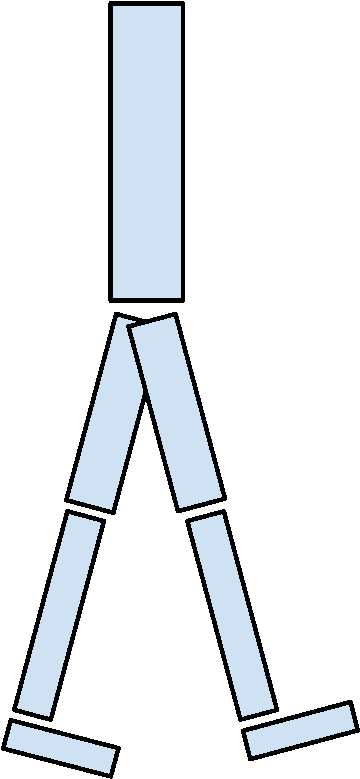
\includegraphics[width=0.2\linewidth]{../images/2D-Biped-crop.pdf} \\
	\caption{\label{figure:2d-biped} 2D planar biped. Each link has $3$ degrees of freedom $\langle x, y, \theta \rangle$.}
\end{figure}

\subsection{Character Construction}

I constructed a $7$ link biped with $21$ degrees of freedom~\ref{figure:2d-biped}. 
The root link is the waist of the character.
In \bulletPhysics links are specified in world coordinates.
After the links are created the constraints between the links are also defined in world coordinates
 
Using the Featherstone algorithm the links between rigid bodies are constructed in a hierarchical fashion. 
To create a new link, a new rigid body is created and then it is added to the system by specifying the id of the parent rigidbody and the child rigidbody. 
For example, if the torso is link $0$ then the left and right thigh links would specify their parent link as $0$.
Links are chained together with \emph{joints} in a method similar to links.
For each joint the parent link needs to be set as well as the child link.
For a hinge joint the axis of rotation also needs to be defined.
Last, the location, in world coordinates, of the joint is defined.
The system also has support for other types of joints but they are not used in this project.

To drive the character each joint has a function to set the current torque for a particular link. 
This torque is automatically applied to both links without the need to enforce the rotation separately.
The link torques will be controlled using Proportional Derivative (PD) controllers.
Each link is driven to a target angle using the formula $\tau = \Kp(\theta_{d}- \theta) - \Kd\dot{\theta} $.
Each non-symmetric joint has different values for \Kp and \Kd.

\begin{comment}
\begin{enumerate}
	\item Constructing a character
	\item Featherstone arrangement
	\item Controlling joints
	\item PD control on these joints
	\item getting a statue
	\item Using different solvers	
\end{enumerate}
\end{comment}

% Onto getting the character to walk

\subsection{Controller States}

The character controller uses a state machine to choose the particular angles the biped should be driving toward. 
There are 4 states and these states are symmetric with respect to the left and right legs of the character.

\begin{comment}
\begin{table}
\centering
	\begin{tabular}{ c | c | c | c | c }
		            & state-0 & state-1 & state-2 & state-3 \\ \hline
         torso      &    0    &    0    &    0    & 0       \\
		 left-hip   &    0    &    0    &    0    & 0       \\
		 left-knee  &    0    &    0    &    0    & 0       \\
		left-ankle  &    0    &    0    &    0    & 0       \\
		 right-hip  &    0    &    0    &    0    & 0       \\
		right-knee  &    0    &    0    &    0    & 0       \\
		right-ankle &    0    &    0    &    0    & 0
	\end{tabular}
	\caption{\label{table:controler-values}}
\end{table}
\end{comment}

%The joint angles for each of the state are listed in Table~\ref{table:controler-values}.
The controller transitions between states for one of two reasons, a specific $\delta t$ has passed since the last transition or there is a new foot contact.

% \todo{description of the states, maybe as picutres}

\subsection{Leg and Torso Control}

To give the biped better walking motion the legs and torso should have an additional control and constraints constraint. 
The first of these is a desired angle for the torso of the biped in world coordinates.
The second is the swing leg of the controller is also driven toward a defined angle in world coordinates.
Last, is a constraint that the torques for the torso (\torqueTorso) and swing leg (\torqueSwing) are equal to the torque generated by the stance leg (\torqueStance). 
This add the constraint $\torqueStance = -\torqueTorso - \torqueSwing$.

\subsection{Feedback Control}

For additional balance control linear feedback is used on the swing leg. This is done in the form

\begin{equation}
\label{equation:feedback-law}
	\feedback = \defaultFeedbackTheta + \distanceFeedbackParam \distance + \velocityFeedbackParam \velocity
\end{equation}

with distance (\distance) and velocity (\velocity) feedback.
The distance \distance is calculated as the distance from the stance foot to the Centre of Motion (\COM), $\distance = -(\location{foot_{stance}} - \location{\COM})$.
The velocity \velocity is simply the velocity of the \COM.

\begin{comment}
\begin{enumerate}
	\item Some math for SIMBICON..
	\item implementing them in BulletPhysics
\end{enumerate}
\end{comment}